\section{LQR controller without payload}
\subsection{full-state feedback controller}

The controller is constructed in Simulink (Figure~\ref{fig:simulink diagram full-state feedback controller}) according to the diagram on page 221 of the course notes. A type 1 full-state feedback was used as its more robust, which is desirable as its controlling a flying object. 

\begin{figure}[H]
	\centering
	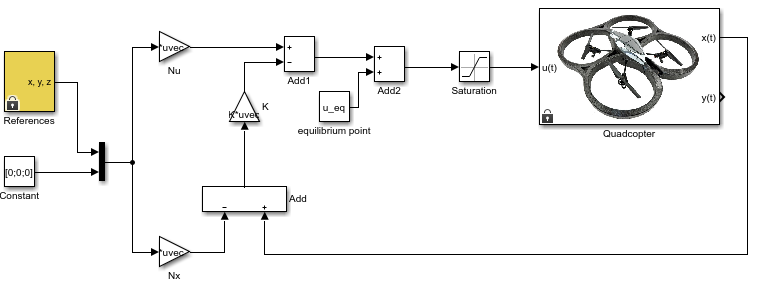
\includegraphics[width=0.5\textwidth]{./LQR_noload/full_state_feedback_simu.png}
	\caption{simulink diagram full-state feedback controller}
	\label{fig:simulink diagram full-state feedback controller}
\end{figure}

The matrix K is calculate with the LQR method as we did in the second exercise session. However in order to do LQR we need a matrix Q and R. As LQR minimizes $J_N = \frac{1}{2} \sum_{k=0}^{N-1}[x_k^TQx_k + u^T_kRu_k] + \frac{1}{2}x_N^TQx_N$. Notice how Q determines the weights given to $x_k$ and and R determines the weights given to $u_k$. 

If Q and R are taken as an diagonal matrix with ones on the diagonal then the quad copter does not have enough power to stay in the air. This is displayed in Figure~\ref{fig:full-state controller with simple diagonal matrices as Q and R}. Its very clear from Figure~\ref{fig:full-state controller with simple diagonal matrices as Q and R demo bad z position} that the controller does not optimize enough on the z axis.

\begin{figure}[H]
	\centering
	\begin{subfigure}[b]{0.3\textwidth}
		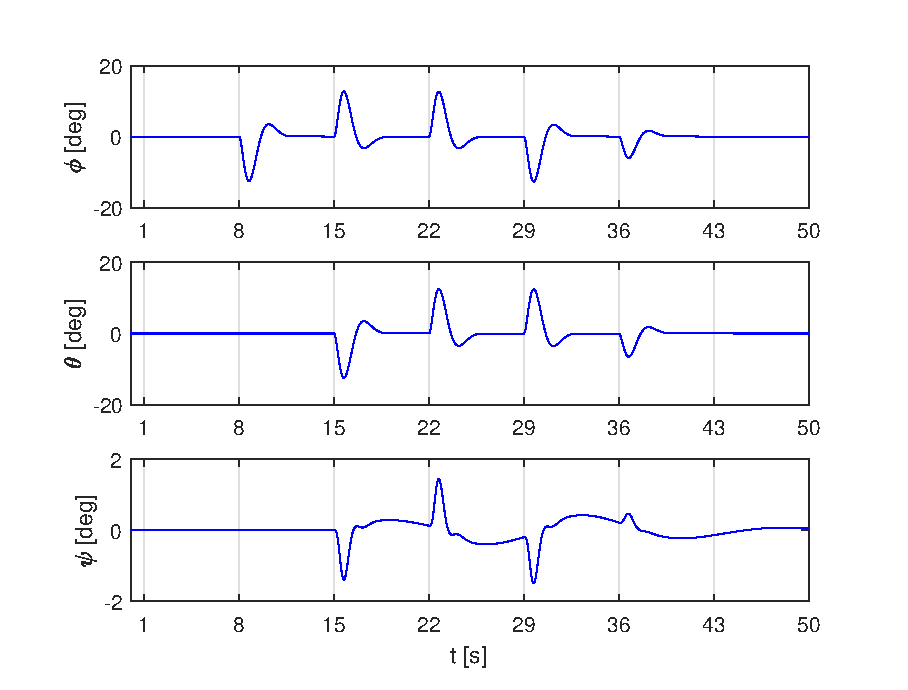
\includegraphics[width=\textwidth]{./LQR_noLoad/full_state/full_state_feedback_first_fig4.eps}
		\caption{angles}
	\end{subfigure}
	\begin{subfigure}[b]{0.3\textwidth}
		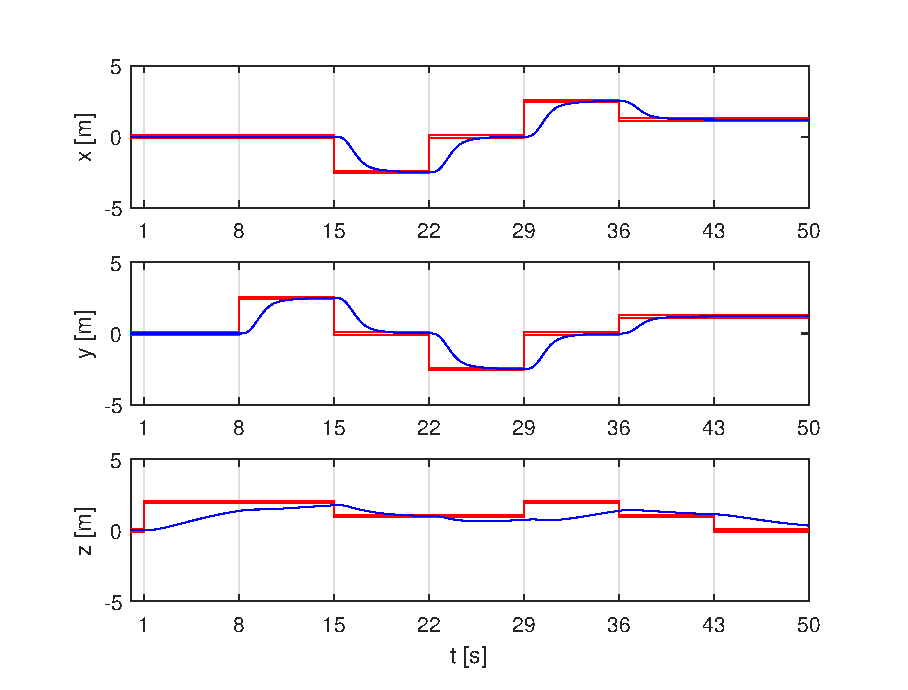
\includegraphics[width=\textwidth]{./LQR_noLoad/full_state/full_state_feedback_first_fig3.eps}
		\caption{position}
		\label{fig:full-state controller with simple diagonal matrices as Q and R demo bad z position}
	\end{subfigure}
	\begin{subfigure}[b]{0.3\textwidth}
		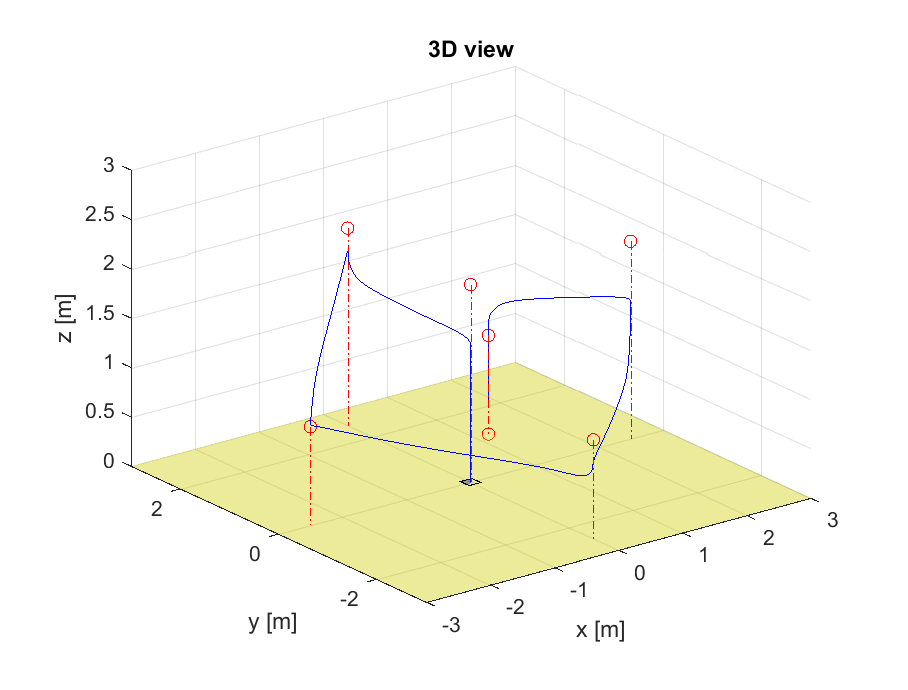
\includegraphics[width=\textwidth]{./LQR_noLoad/full_state/full_state_feedback_first_fig2.eps}
		\caption{track}
	\end{subfigure}
	\caption{full-state controller when Q and R are unit matrices}\label{fig:full-state controller with simple diagonal matrices as Q and R}
\end{figure}

In order to get a proper controller we need to put way more weight on the position z in the optimization problem. This is done by increasing a value in Q, as the z coordinate is an state. 

$$ 
Q=
\begin{bmatrix}
1 & 0 & 0 & 0 & ... \\
0 & 1 & 0 & 0 & ...\\
0 & 0 & 1 & 0 & ... \\
0 & 0 & 0 & 1 & ... \\
... & ... & ... & ... & ... 
\end{bmatrix}
=>
\begin{bmatrix}
1 & 0 & 0 & 0 & ... \\
0 & 1 & 0 & 0 & ...\\
0 & 0 & 10^2 & 0 & ... \\
0 & 0 & 0 & 1 & ... \\
... & ... & ... & ... & ... 
\end{bmatrix}
$$

\begin{figure}[H]
	\centering
	\begin{subfigure}[b]{0.3\textwidth}
		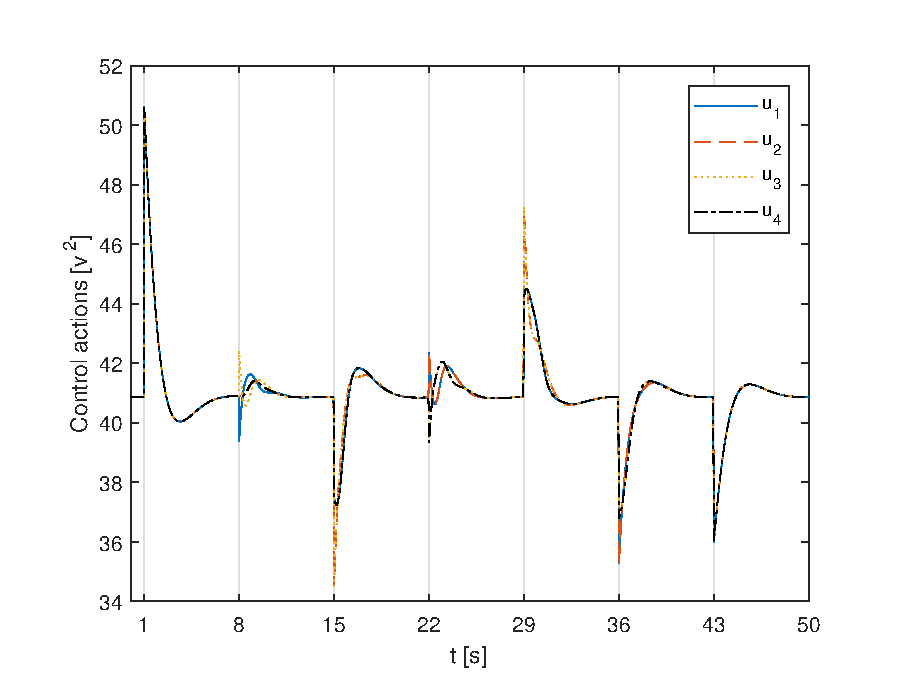
\includegraphics[width=\textwidth]{./LQR_noLoad/full_state/full_state_feedback_increased_z_fig5.eps}
		\caption{input voltages motors}
		\label{fig:full-state controller with low voltage}
	\end{subfigure}
	\begin{subfigure}[b]{0.3\textwidth}
		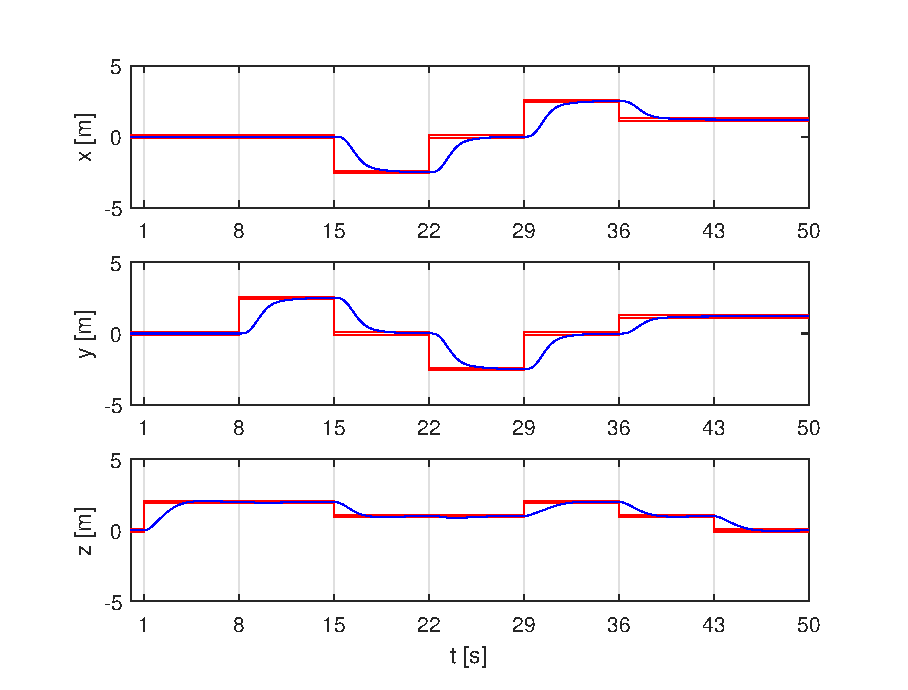
\includegraphics[width=\textwidth]{./LQR_noLoad/full_state/full_state_feedback_increased_z_fig3.eps}
		\caption{position on each axis}
	\end{subfigure}
	\begin{subfigure}[b]{0.3\textwidth}
		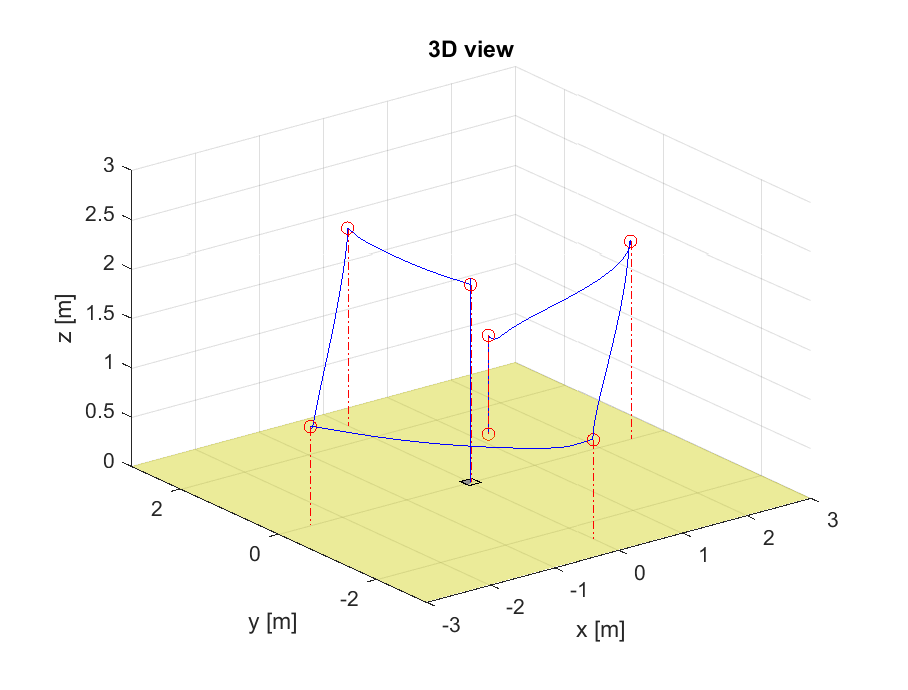
\includegraphics[width=\textwidth]{./LQR_noLoad/full_state/full_state_feedback_increased_z_fig2.eps}
		\caption{3D position}
	\end{subfigure}
	\caption{full-state controller with adjusted Q an unit matrix as R }\label{fig:full-state controller with adjusted Q matrix but a unit matrix as R}
\end{figure}

Figure~\ref{fig:full-state controller with adjusted Q matrix but a unit matrix as R} contains the results of the full state controller with the adjusted Q matrix. The quad-copter does reach all its checkpoint but the input voltages on the motors are rather low. 

Lowering the values of R  will result in higher voltages and so an increase speed. But keeping robustness in mind R must still be sufficiently large to avoid oscillating or extremely fast changes in voltages. A diagonal value of 0.1 seems to be reasonable for R, this is illustrated in Figure~\ref{fig:full-state controller with proper diagonal matrices as Q and R}.The adjustment of R improves the average time from 3.736 to 3.214 s. Notice how the voltage also get lower in Figure~\ref{fig:full-state controller with proper diagonal matrices as Q and R - voltages}, the controller is way more nervous then in Figure~\ref{fig:full-state controller with low voltage}.
\begin{figure}[H]
	\centering
	\begin{subfigure}[b]{0.3\textwidth}
		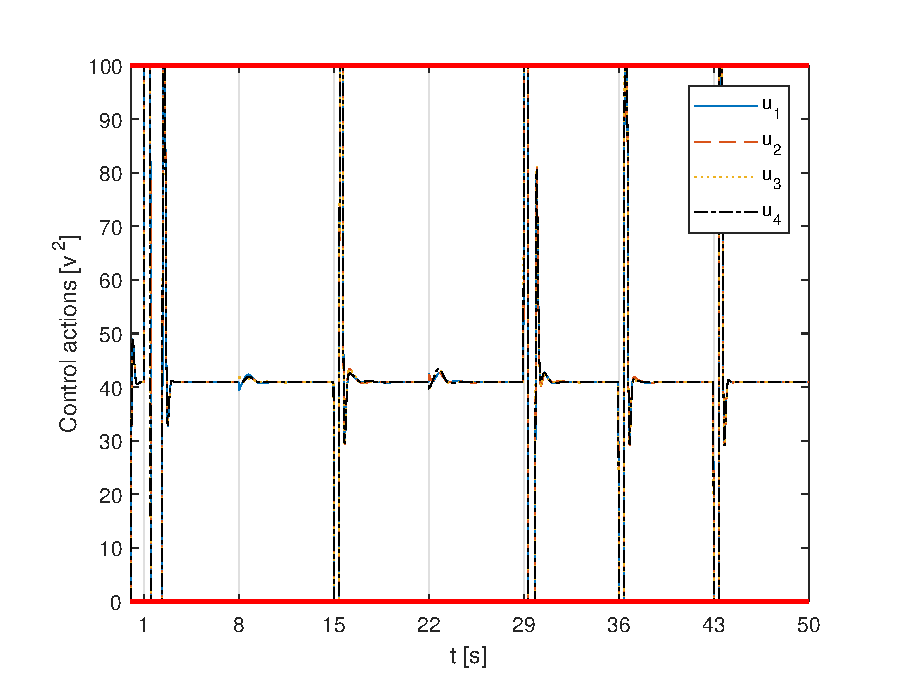
\includegraphics[width=\textwidth]{./LQR_noLoad/full_state/full_state_feedback_final_fig5.eps}
		\caption{angles}
		\label{fig:full-state controller with proper diagonal matrices as Q and R - voltages}
	\end{subfigure}
	\begin{subfigure}[b]{0.3\textwidth}
		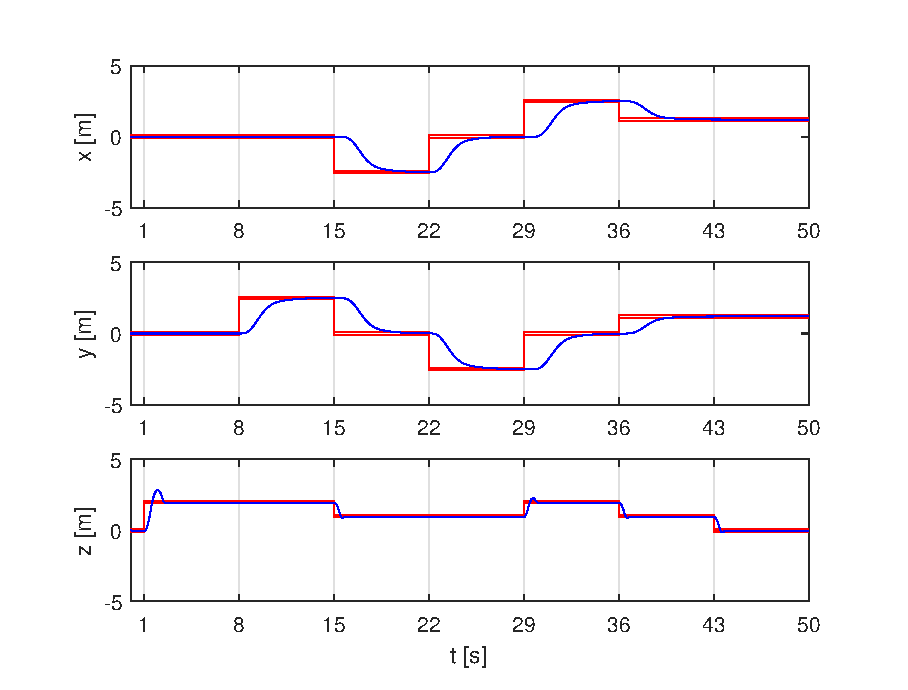
\includegraphics[width=\textwidth]{./LQR_noLoad/full_state/full_state_feedback_final_fig3.eps}
		\caption{position}
	\end{subfigure}
	\begin{subfigure}[b]{0.3\textwidth}
		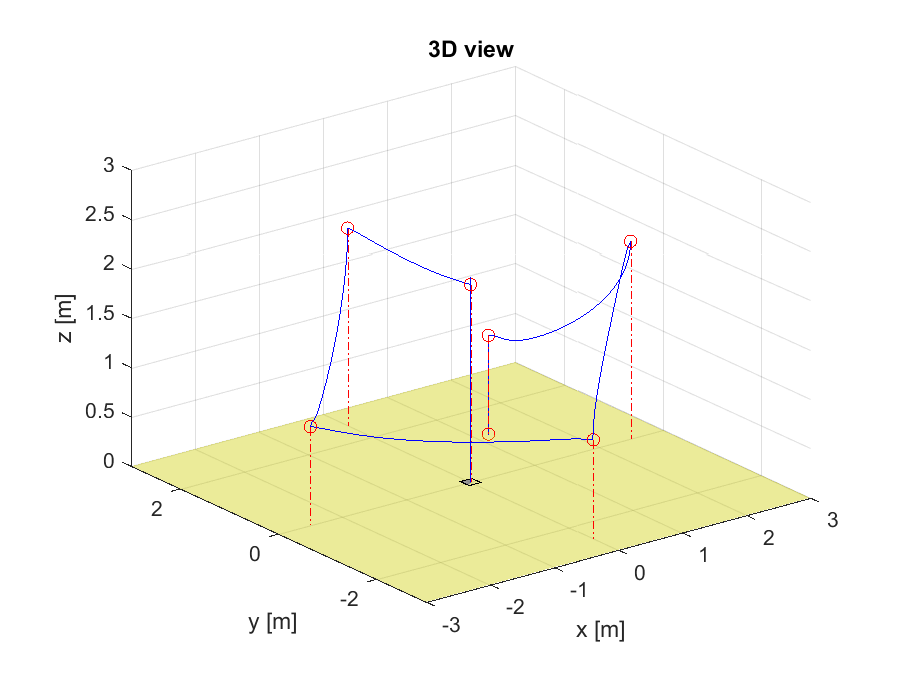
\includegraphics[width=\textwidth]{./LQR_noLoad/full_state/full_state_feedback_final_fig2.eps}
		\caption{track}
	\end{subfigure}
	\caption{full-state controller with proper diagonal matrices as Q and R}\label{fig:full-state controller with proper diagonal matrices as Q and R}
\end{figure}
\subsubsection{Final weight matrices}

$$
Q=\begin{bmatrix}
1 & 0 & 0 & 0 & 0 & 0 & 0 & 0 & 0 & 0 & 0 & 0 \\
0 & 1 & 0 & 0 & 0 & 0 & 0 & 0 & 0 & 0 & 0 & 0 \\
0 & 0 & 10^2 & 0 & 0 & 0 & 0 & 0 & 0 & 0 & 0 & 0 \\
0 & 0 & 0 & 1 & 0 & 0 & 0 & 0 & 0 & 0 & 0 & 0 \\
0 & 0 & 0 & 0 & 1 & 0 & 0 & 0 & 0 & 0 & 0 & 0 \\
0 & 0 & 0 & 0 & 0 & 1 & 0 & 0 & 0 & 0 & 0 & 0 \\
0 & 0 & 0 & 0 & 0 & 0 & 1 & 0 & 0 & 0 & 0 & 0 \\
0 & 0 & 0 & 0 & 0 & 0 & 0 & 1 & 0 & 0 & 0 & 0 \\
0 & 0 & 0 & 0 & 0 & 0 & 0 & 0 & 1 & 0 & 0 & 0  \\
0 & 0 & 0 & 0 & 0 & 0 & 0 & 0 & 0 & 1 & 0 & 0 & \\
0 & 0 & 0 & 0 & 0 & 0 & 0 & 0 & 0 & 0 & 1 & 0 & \\
0 & 0 & 0 & 0 & 0 & 0 & 0 & 0 & 0 & 0 & 0 & 1 & \\
0 & 0 & 0 & 0 & 0 & 0 & 0 & 0 & 0 & 0 & 0 & 0 & \\
0 & 0 & 0 & 0 & 0 & 0 & 0 & 0 & 0 & 0 & 0 & 0 & \\
0 & 0 & 0 & 0 & 0 & 0 & 0 & 0 & 0 & 0 & 0 & 0 & \\
\end{bmatrix}
$$
$$
R=\begin{bmatrix}
0.1 & 0 & 0 & 0 \\
0 & 0.1 & 0 & 0 \\
0 & 0 & 0.1 & 0 \\
0 & 0 & 0 & 0.1 \\
\end{bmatrix}
$$

